% !TEX root = main.tex

\chapter{Design and simulation of the addressing setup}
\section{Addressing system overview and requirements}
\section{Objective and AOD}
\section{Addressing setup}

\begin{figure}[H]
\centering
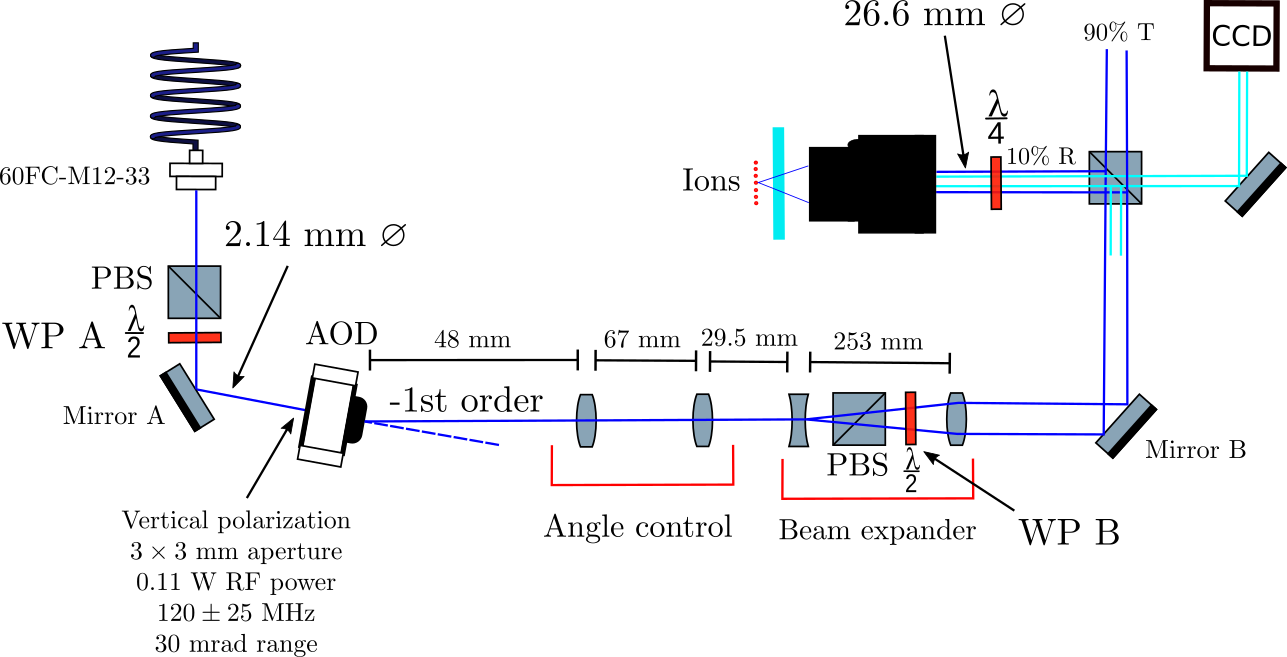
\includegraphics[width=\textwidth]{img/setup}
\caption{Setup scheme}
\end{figure}


\begin{figure}[H]
\centering
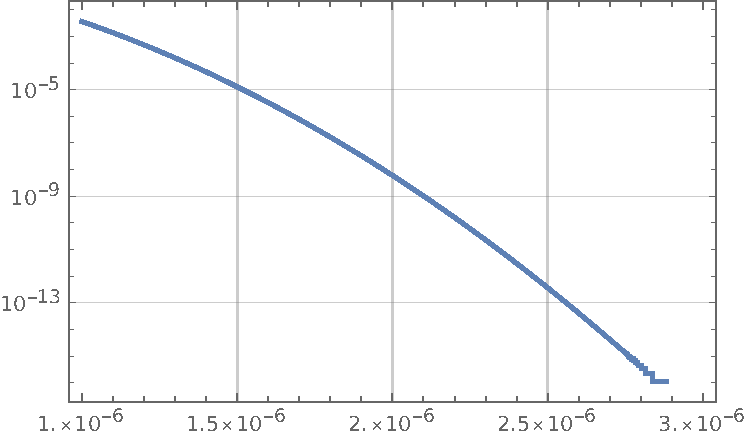
\includegraphics[width=\textwidth]{img/Plosses}
\caption{Losses on the compensation electrodes vs beam waist}
\end{figure}
\begin{figure}[H]
\centering
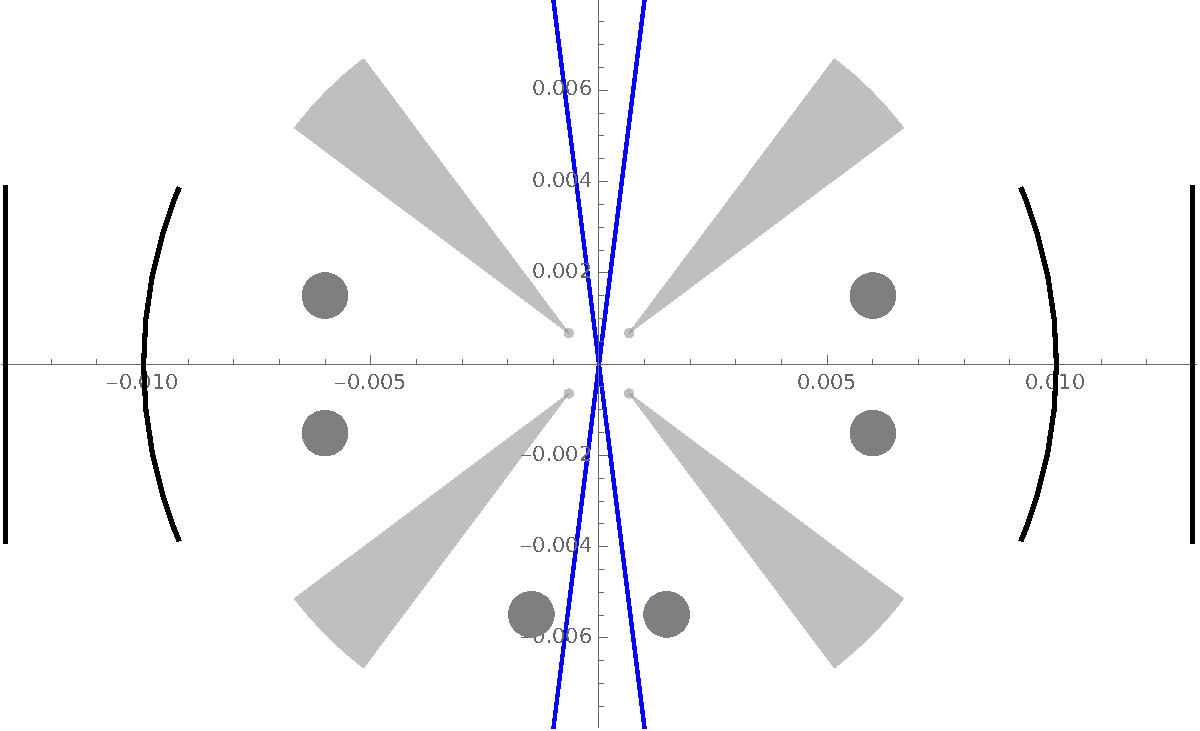
\includegraphics[width=\textwidth]{img/clipping}
\caption{Clipping on compensation electrodes}
\end{figure}

- Scheme of real setup \\
- Alignment process
